\documentclass{article}
\usepackage{lmodern}
\usepackage[utf8]{inputenc}
%\usepackage[spanish, activeacute]{babel}
\usepackage{mathtools}
\usepackage{amsthm}
\usepackage{amssymb}
\usepackage{tikz}
\usepackage{xcolor}
\usepackage{enumitem}
\usepackage{ragged2e}
\renewcommand{\proofname}{Dem:}

\begin{document}
  \begin{justify} %Pregunta 1
    1.Sea $G$ la gráfica tal que $V(G) = {v_1,v_2,...,v_9}$ y donde $v_i ady_G v_j$ si y sólo si $i \leq \lfloor \frac{j}{2} \rfloor $ o $j \leq \lfloor \frac{i}{2} \rfloor $. Encuentra el orden, tamaño, el grado mínimo y el grado máximo de $G$.
    \ttfamily{
      \begin{enumerate}
      \item Encontrar el orden. \\
        Sabemos que el ordén de una gráfica es el número de vértices \\
        $ \Longrightarrow V(G) = {v_1, v_2, ..., v_9} = 9$ vertices. \\
        $\therefore $ Su orden es de 9. $\left| V(G) \right|$.
      \item Encontrar el tamaño. \\
        Sabemos que el tamaño de una gráfica es el número de aristas. \\
        $\Longrightarrow $ Se cuentan las conexiones que cumplan la condición dada. \\
        $v_i ady_G v_j \Longleftrightarrow i \leq \lfloor \frac{j}{2} \rfloor $ o $j \leq \lfloor \frac{i}{2} \rfloor $ \\

        Para evitar repetir el conteo de alguna arista tomamos los valores $i<j$ \\
        $\Longrightarrow $ Las asistas que satisfacen $i \leq \lfloor \frac{j}{2} \rfloor $ son: \\
        \begin{align}
          1 \leq i \leq \lfloor \frac{j}{2} \rfloor \\
        \end{align}
        \begin{itemize}
          \item Con $j = 2$ \\
          Ya que, si $j=1$ no cumple la fórmula para algún indice, dado que $i \leq \lfloor \frac{1}{2} \rfloor = i \leq 0.5 \Longrightarrow i \leq 0$, pero no existe ningún indice $i$ que cumple eso. \\
          $\Longrightarrow $ $i \leq \lfloor \frac{2}{2} \rfloor$ $\Longrightarrow i \leq 1$ Y esto si se cumple.
          $\therefore$ $(v_1 ady_G v_2)$ \\
        \item Con $j = 3$ \\
          $i \leq \lfloor \frac{3}{2} \rfloor$ $\Longrightarrow i \leq 1.5 \\ \Longrightarrow i \leq 1$, y esto nuevamente se cumple. \\
          $\therefore (v_1 ady_G v_3)$ \\
        \item Con $j = 4$ \\
          $i \leq \lfloor \frac{4}{2} \rfloor$ $\Longrightarrow i \leq 2 \\$ \mbox{Y esto nuevamente se cumple, pero esta vez con $i=1  \land i=2. $\\}
          $\therefore (v_1 ady_G v_4) \land (v_2 ady_G v_4)$ \\

        \item Con $j = 5$ \\
          $i \leq \lfloor \frac{5}{2} \rfloor$ $\Longrightarrow i \leq 2.5 \Longrightarrow i \leq 2 \\$ \mbox{Ent. las adyacencias posibles son:}\\
          $(v_1 ady_G v_5) \land (v_2 ady_G v_5)$ \\
          \newpage
        \item Con $j= 6$ \\
          $i \leq \lfloor \frac{6}{2} \rfloor$ $\Longrightarrow i \leq 3 \\$ \mbox{Ent. las adyacencias posibles son:}\\
          $(v_1 ady_G v_6) \land (v_2 ady_G v_6) \land (v_3 ady_G v_6)$\\
        \item Con $j = 7$ \\
          $i \leq \lfloor \frac{7}{2} \rfloor$ $\Longrightarrow i \leq 3.5 \Longrightarrow i \leq 3 \\$ \mbox{Ent. las adyacencias posibles son:}\\
          $(v_1 ady_G v_7) \land (v_2 ady_G v_7) \land (v_3 ady_G v_7)$ \\
        \item Con $j= 8$ \\
          $i \leq \lfloor \frac{8}{2} \rfloor$ $\Longrightarrow i \leq 4 \\$ \mbox{Ent. las adyacencias posibles son:}\\
          $(v_1 ady_G v_8) \land (v_2 ady_G v_8) \land (v_3 ady_G v_8) \land (v_4 ady_G v_8)$ \\
        \item Con $j = 9$ \\
          $i \leq \lfloor \frac{9}{2} \rfloor$ $\Longrightarrow i \leq 4.5 \Longrightarrow i \leq 4 \\$ \mbox{Ent. las adyacencias posibles son:}\\
          $(v_1 ady_G v_9) \land (v_2 ady_G v_9) \land (v_3 ady_G v_9) \land (v_4 ady_G v_9)$ \\
        \end{itemize}
        Ent. sumando las aristas tenemos que: \\
        \begin{align}
          1+1+2+2+3+3+4+4 = 20\\
        \end{align}
        $\therefore $ su tamaño es de 20.
      \item Grado máximo \\
        Para esto, el grado $d(V) $ es la cantidad de vecino $N(v)$. Entonces, con lo que ya tenemos de los incisos anteriores, buscamos el vértice con la mayor cantidad de vecinos.\\
        Se puede observar como $v_1$ es adyacente a todos los demás vertices de $V$\\
        $\therefore  \d(v_1) = 8$ y como es el único que cumple ser adyacente a todos los demás, podemos decir que es de grado máximo.
        $\therefore \Delta(G) = 8$
      \item Grado mínimo \\
        Notese que, $V_5$ es adyacente unicamente a $v_1 \land v_2 $. \\
        Por lo tanto, $ªd(v_5) = 2$ este vértice sería el único en ser a dos vértices, y al ser no existir ningún otro con algún grado menor.
        Entonces podemos decir que es el grado mínimo de $G$.\\
        $\therefore \delta(G) = 2$
      \end{enumerate}
      }
\end{justify}

\newpage
\begin{justify} %Problema 2
  2.Encuentra el \underline{complemento} de la gráfica del \underline{Ejercicio 1}. Determina su orden, tamaño, grado mínimo y máximo. \\
  \ttfamily{
    Sea $G$ la gráfica del \underline{Ejercicio 1} con \\
    \begin{align}
      \left| V(G) \right| = 9    \land   \left| E(G) \right| = 20 \\
    \end{align}
    Denotamos a su complemento como, $\hat{G}$.
    \begin{itemize}
    \item a) Orden \\
      El complemento tiene el mismo conjunto de vértices. \\
      $\therefore     \left| V(\hat{G}) \right| = 9$ 
    \item b) Tamaño \\
      \noindent\fbox{
       \begin{minipage}{\textwidth}
         \textbf{Observación: } Si $G$ es una gráfica de orden n y tamaño m. Entonces, $\hat{G}$ es una gráfica de orden n y tamaño: $( \frac{n}{2} ) -m$. \\
       \end{minipage}
       }
     Entonces, sustituyendo $G$ para obtener el tamaño de $\hat{G}$: \\
     $( \frac{n}{2} )- m$ , $\Longrightarrow ( \frac{9}{2} ) = 36 $ , Como G tiene 20 aristas, ent. \\
     $36-20 = 16$   \\ $\therefore \left| E(\hat{G}) \right| = 16$
   \item C) Grado mínimo y màximo \\
     Recordando que el conjutnode aristas del complemento de G, es decir, $\hat{G}$ es: ${uv | u,v \in V, u \neq v} \ E(G)$. Esto implica que un
     vertice $u$ sera adyacente en $\hat{G}$ a todos aquellos vertices con los que no eran adyacentes en $G$. \\

     Cada vertice puede tener a lo más n-1 vecinos como en este caso $n = 9 \Longrightarrow n-1 = 8 $ \\
     $\therefore$ para cada vertice $u$. \\
     \begin{align}
       d(\hat{G}) = 8 - d(G(V))
     \end{align}
     Para el grado máximo de $\hat{G}$ se obtiene restando el grado mínimo de G.
     \begin{align}
       \Delta(\hat{G}) &= (n-1) - \delta(G) \\
       \Longrightarrow \Delta(\hat{G}) &= (9-1) - 2\\
       &= 8-2\\
       &= 6\\
         \therefore \Delta(\hat{G}) &= 6\\
     \end{align}
     Para el grado mínimo de $\hat{G}$ se obtiene restando el grado máximo de $G$. \\
     \begin{align}
       \delta(\hat{G}) &= (n-1) - \Delta(G) \\
       Sustituyendo \\
       \delta(\hat{G}) &= (9-1) - 8\\
                       &= 8-8 \\
                       &=0 \\
       \therefore \delta(\hat{G}) &= 0
     \end{align}
    \end{itemize}
    }
  \end{justify} %Fin del problema 2
  \begin{justify} %Inicio del problema 3
    3. Demuestra que toda gráfica $G$ de orden n es isomorfa a una subgráfica de la gráfica completa $K_n$
    \begin{proof}
      Sea $G$ una gráfica de orden n, la podemos escribir de la siguiente manera: $V(G) = (v_1, v_2, ..., v_n) $ y $K_n$ al ser una gráfica
      una gráfica completa sabemos por su definición que $\forall$ par de vértices $u_i,u_j \in V(K_n)$, siempre existe una arista que los une
      $ e_i = u_i, u_j$ \\
      Como ambas gráficas poseen orden $n$, podemos escribir $\lambda$ una función biyectiva. \\
      $\Longrightarrow $ Sea $H$ una subgráfica de $K_n$ donde tengan el mismo número de vertices. 
      Donde la arista $e_i $ existe si y solo si existe $e\prime = v_i v_j $ en $G$. \\
      Por la forma en la que esta definida $H$ y la función $\lambda$, se cumple que $v_i$ es adyacente a $v_j$ si y solo si $\lambda(v_i)$
      $adyacente a \lambda(v_j)$ en $H$.\\
      $\therefore$ la función $\lambda$ es isomorfa entre $G$ y $H$. \\
      $\therefore G$ es isomorfa a una subgráfica de $K_n$. 
    \end{proof}
  \end{justify} %Fin del problema 3
  \newpage
   4. Muestre lo siguiente: %Problema 4
  \begin{enumerate}
  \item $(a)$ Demuestra que toda subgráfica inducida de una gráfica completa es completa. \\
    \begin{proof}
      Sea $G = k_n$ una gráfica completa $\land G'=(V',E') $subgráfica inducida de $k_n $. Por la definición de \underline{gráfica inducida}.
      Tenemos que $V'(G') \subseteq V(G)$ y tambien sabemos que $E' = {(uv)\in E | (u,v)\in V'}$. \\

      Entonces. Sean $v_1,v_2 \in V' tq v_1 \neq v_2$ \\
      $\Longrightarrow$ Como $V' \subseteq V$.Entonces, $v_1,v_2 \in V$, Entonces tiene que existe arista $(v_1v_2)\in E$.\\
      Por la definición de gráfica inducida si ambos vértices pertecen a $V$, entonces la arista $(v_1v_2)\in E'$. \\
      $\therefore G'$ es gráfica completa.
    \end{proof}

  \item $(b)$ Demuestra que la suma de gráficas completas, es completa. \\
    \begin{proof}
      Sea $G_1 = (V_1,E_1) y G_2= (V_2,E_2) $ gráficas completas. \underline{$PD$} $G = G_1+G_2$ es una gráfica completa. \\
      Para el caso de los vértices de $V(G)$, sabemos por definición de suma que: $V(G) = V(G_1)+V(G_2)$.\\
      Ahora Para sacar el valor de $E(G)$, se tiene lo sig. por definición de suma. \\
      \begin{equation}
        E(G) = E_1 \cup E_2 \cup {uv | u\in V(G_1) \land v\in(G_2)}
      \end{equation}
      $\Longrightarrow$ Sea $u_1,u_2 \in V(G)$. Los cual por la definición tenemos 3 casos posibles.
      \begin{description}
      \item[caso 1] Si $u_1,u_2 \in V(G_1)$. Como $G_1$ es completa. \\Entonces, $(u_1u_2)\in E(G_1)$. Por definición de suma.
        $E(G_1) \subseteq E(G) $ $\therefore (u_1u_2)\in E(G)$ \\
      \item[caso 2] Si $u_1,u_2 \in V(G_2)$. Este se sigue de manera analoga al primer caso. \\
      \item[caso 3] Supongamos s.p.g que:  $u_1 \in V(G_1) \land u_2 \in V(G_2)$. Por la definición de suma se agregan a $E(G)$ todas las aristas
        entre ambos vértices. $\therefore$ $u_1u_2 \in E(G)$.\\ 
      \end{description}
      Se puede observar que los 3 casos se cumplen. \\
      $\therefore$ la suma de gráficas completas, es completa. \\

    \end{proof}
    
    
  \end{enumerate}
  
  % Problema 5
  \begin{justify}
    $5$. Determina si la siguientes sucesiones son las sucesiones de grados de una gráfica.
    \begin{enumerate}[label=\alph*)]
    \item[a)] $S : 4, 4, 3, 2, 2$\\
      Vamos a probar si se pueden sacar las sucesiones basados en la sumatoria de grados. \\
      \ttfamily{
        \noindent\fbox{%
          \begin{minipage}{\textwidth}
            \textbf{Hint:} $\sum_{i=1}^{n} d_G(V_i) = 2m$
          \end{minipage}
        }
      }
      Podemos observer que en este caso. \\
      \begin{equation}
        4+4+3+2+2 = 15
      \end{equation}
      Y 15 es número impar. Aplicando nuestra sumatoria, para que se cumpla la igualda con $2m$ forzosamente la suma de grados tiene
      que ser impar. \\
      $\therefore$ La prmera sucesión no es sucesión de grados de una gráfica.
    \item[b)] $S : 5, 5, 4, 4, 4, 3, 2, 1$ \\
      Primero aplicando lo que sabemos de la sumatoria.
      $Longrightarrow$ \\
      \begin{equation}
        5+5+4+4+4+3+2+1 = 28
      \end{equation}
      Claramente es un número par. Entonces si podría llegar a ser sucesión de grados par alguna gráfica. \\
      \underline{Verifiquemos} \\
      \texttt{
        Eliminamos $d_1 = 5$ y restamos 1 a los siguientes 5 terminos. \\
        $S_2 = 4+3+3+3+2+2+1$ \\
        Eliminamos $4$ y restamos 1 a los siguientes 4 terminos. \\
        $S_3 = 2+2+2+1+2+1 : S_3 = 2+2+2+2+1+1$  \\
        Eliminamos $2$ y restamos 2 a los siguientes 2 terminos. \\
        $S_4 = 1+1+2+1+1 : S_4 = 2+1+1+1+1 $\\
        Eliminamos $2$ y restamos 2 a los siguientes 2 terminos. \\
        $S_5 = 0+0+1+1 : S_5 = 1+1+0+0$ \\
        Eliminamos $1$ y restamos 1 al siguiente termino. \\
        $S_6 = 0+0+0$ \\
        Como el proceso termino en ceros, la sucesión si es sucesión de grados para alguna gráfica. \\
      }
    \item[c)] $S : 6, 5, 5, 4, 3, 3, 2, 1 $\\
      Primero apliquemos la fórmula de sumatoria: \\
      \begin{equation}
        6+5+5+4+3+3+2+1 = 29 \\
      \end{equation}
      Por el mismo argumento que \textbf{a)}, al ser impar no puede ser sucesión de grados para alguna gráfica. \\
    \end{enumerate}
    
  \end{justify}

  % Problema 6
  \newpage
  \begin{justify}
    6. Dibuja una gráfica con las sucesiones de grados del \underline{Ejercicio 5} en los casos en que
    sean la sucesión de grados de una gráfica.
    Vamos a tomar la gráfica del ejercicio \textbf{b)}, dado que fue la única que cumplio. \\
    $\Longrightarrow$ tenemos que $S :  5, 5, 4, 4, 4, 3, 2, 1 $ \\
    Sea $G = (V,G)$ se puede observer que tenemos 8 vertices. Entonces $V = {a,b,c,d,e,f,g,h}$ \\
    Ahora asignando los grados tenemos que. \\
    $a = 5, b = 5, c = 4, d = 4, e = 4, f = 3, g = 2, h = 1$\\
    G:\\
    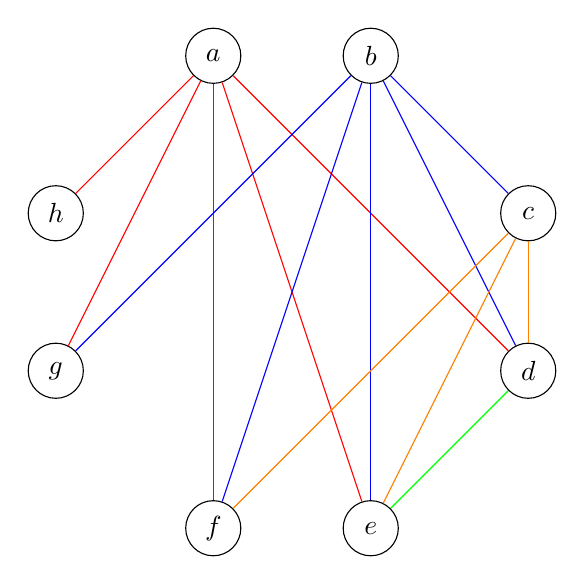
\begin{tikzpicture} %Grafica 1
      [
      node/.style={circle, draw, minimum size=0.7cm, inner sep=0pt}
      ]
      \node[node] (a) at (-1,3) {$a$};
      \node[node] (b) at (1,3) {$b$};
      \node[node] (c) at (3,1) {$c$};
      \node[node] (d) at (3,-1) {$d$};
      \node[node] (e) at (1,-3) {$e$};
      \node[node] (f) at (-1,-3) {$f$};
      \node[node] (g) at (-3,-1) {$g$};
      \node[node] (h) at (-3,1) {$h$};
      \begin{scope}[draw = red]
        \draw (a) -- (h);  \draw (a) -- (g); \draw (a) -- (f); \draw (a) -- (e); \draw (a) -- (d);
      \end{scope}
      \begin{scope}[draw = blue]
        \draw (b) -- (c);  \draw (b) -- (g); \draw (b) -- (f); \draw (b) -- (e); \draw (b) -- (d);
      \end{scope}
      \begin{scope}[draw = orange]
        \draw (c) -- (d);  \draw (c) -- (e); \draw (c) -- (f);
      \end{scope}
      \begin{scope}[draw = green]
        \draw (d) -- (e);
      \end{scope}
      
      
      
    
      
\end{tikzpicture}
  \end{justify}
  
  \begin{justify} %7/ 8
  Sean $G_1$ y $G_2$ gráficas de ordenes $n_1$ y $n_2$; y de tamaños $m_1$ y $m_2$, respectivamente.\\
  \textbf{7. Determina el orden y el tamaño de $G_1 \square G_2$}
  \end{justify}
  \begin{proof}
    Sean $G_1 = (V_1, E_1) \land  G_2 = (V_2,E_2)$ 
    Para determinar el orden de $G_1 \square G_2$. Se obtiene como el producto de los conjuntos de vértices de $V_1$ y $V_2$. \\
    $\Longrightarrow$   $ n = \left| V_1 \times V_2 \right| = |V_1| \cdot |V_2| = n_1 \cdot n_2$ \\
    Para determinar el tamaño de $G_1 \square G_2$. Se tiene que obtener el conjunto de aristas.\\ \{$(v_1,v_2)(\hat{v_1}, \hat{v_2}) |
    v_1 adyG_1 \hat{v_1} $ y $ v_2 = \hat{v_2} $ o $ v_2 adyG_2 \hat{v_2} $ y $ v_1 = \hat{v_1}$\} \\
    \begin{itemize}
    \item Existen entonces $m_1$ aristas en $G_1$ que se generan $n_2$ veces.\\
      $\therefore $ Esto nos da  $m_1 \cdot n_2 $.\\
    \item Existen $m_2$ aristas en $G_2$ que se generan $n_1$ veces.
      $ \therefore $ Esto nos da $m_2 \cdot n_1$. \\
    \end{itemize}

    Para obtener el tamaño de $G_1 \square G_2$. Entonces $m = |E(G_1) + E(G_2)| $ \\
    $\therefore$ el tamaño de $G_1 \square G_2$ es $m = n_2m_1 + n_1m_2 $
  \end{proof}
  % 8.
  \textbf{8. Determina el orden y el tamaño de $G1 \times G2$.} \\
  \begin{justify}
    Sean $n_1$ y $n_2$ ordenes y tamaños $m_1$ y $ m_2$ de $G_1$ y $G_2$  respectivamente,
    el orden de $G_1 \times  G_2 $ es $n_{G_1} \times n_{G_2} = n_1 \times n_2$ \\
    El tamaño de $G_1 \times G_2 $ por \textit{def.} del producto cruz. \\
    \ttfamily{
      \noindent\fbox{%
        \begin{minipage}{\textwidth}
          \textbf{\textit{Producto Cruz}:} $E(G_1 \times G_2) = {(u_1,u_2), (v_1,v_2) | u_1 ady_G v_1 \land u_2 ady_G v_2}$  \\
        \end{minipage}
      }
    }
    Dado que cada arista $(u_1,u_2) \in E(G_1) $ y  $(v_1,v_2) \in E(G_2) $ por la \textit{def.} de Producto cruz, existe una arista. \\
    Entonces, el producto cruz de ambas serán todas las posibles combinaciones de las aristas originales. \\
    $\therefore E(G_1 \times G_2) = m_1 \times m_2$ 
  \end{justify}
    
    % 9.
    \begin{justify}
      9. Sea $G$ una gráfica de orden $n$ y tamaño $m$. Demuestra que si $m > \leq \lfloor \frac{n}{2} \rfloor$\\
      entonces $G$ contiene trayectoria de longitud al menos dos.
    \end{justify}
    \begin{proof}
      Sea $G = (V,E)$ gráfica con orden $n$ y tamaño $m$. Si $m > \leq \lfloor \frac{n}{2} \rfloor$.\\ \textbf{PD.} longitud de la trayectoria
      $\geqslant 2$. \\
      Demostración por \underline{Contrapuesta} \\
      Supongamos que $G$ no tiene una longitud $\geqslant 2$. \\
      Entonces todos los vértices de $G$ pueden tener a lo más 1 vecino. Dado que si algún vértice tuviera más de un vecino, tendríamos que
      su trayectoria sería de almenos 2. \\
      Utilizando la sumatoria de grados, entonces tenemos que:
      \begin{align}
        \sum_{v \in V(G)}^{n} d(v) = 2m \\
      \end{align}
      
      \underline{Como cada } d(v) $\leq$ 1, entonces la suma tiene que ser a lo más n. \\
      Despejando $m$ en la ecuación de abajo, tenemos que: 
      \begin{align}
        n = 2m\\
        \frac{n}{2} \leq m
      \end{align}
    \end{proof}
    \newpage
    % 10.
    \begin{justify}
      10.Sea $G$ una gráfica de orden $n$, acíclica y de tamaño $n-1$. Demuestra que $G$ tiene al menos una hoja.
      \begin{proof} \underline{Contradicción}
        Supongamos que $G$ no tiene hojas. \\
        Entonces todos los vertices tienen grado a lo más $\geq$ 2. \\
        Como tiene orden $n$ y es acíclica, por la sumatoria de grados, tendríamos que como mínimo. \\
        \begin{equation}
          2m = \sum_{v \in V(G)}^ n d(v) = 2n
        \end{equation}
        Pero sabemos que el tamaño es $n-1$ \\
        $\Longrightarrow 2(n-1) = 2n$ $\bot$ \\
        Esto no puede ocurrir. \\
        $\therefore$ $G$ tiene al menos una hoja.

      \end{proof}
    \end{justify}
  11. Demuestra que un \textit{árbol} es una gráfica \textit{bipartita}.
  
  \begin{proof}
    \ttfamily{
      Sea $G$ un árbol y \underline{PD} que $G$ es gráfica bipartita \\
      Podemos aplicar el siguiente teorema: \\
      
      \noindent\fbox{%
        \begin{minipage}{\textwidth}
          \textbf{Teorema:} $G$ es bipartita si y solo si no tiene ciclos de longitud impar
       \end{minipage}
     }
   }
   Aplicando su regreso en $G$, al ser un árbol este no posee ningún ciclo al ser acíclica. \\
   $ \Longrightarrow $ no posee ciclos de longitud impar\\
   $\therefore$ $G$ es bipartita.
 \end{proof}
 
 12. Determina el número de hojas de un árbol $m$-ario de orden $n$. \\
 
 \begin{proof}
   \ttfamily{
     Sea $T$ un árbol $m$-ario de orden $n$ \\
     Por su definición de ser $m$-ario este posee un un vértice de grado $m$ y el resto de sus vértices posee grado m+1 o son hojas. \\
     En caso de ser hojas sabemos que su grado será de 1. \\
     
     Sea $l$ los vértices de grado $m+1$, como $T$ es de ordén $n$ y es $m$-ario, podemos decir que: \\
     $n = ml + 1$ \\
     Ahora vamos a denotar al conjunto de vértices que son hojas como $h$ \\
     $ \Longrightarrow $ $ l = n-h $
     Podemos reescribir la fórmula de $n$ como: \\
     \begin{align}   
       n &= m(n-h) +1 \\
       n &= mn - mh +1 \\
       mh &= mn - n +1 \\
       h &= \frac{mn-n+1}{m} \\
       h &= \frac{n(m-1) +1}{m}
       \\
    \end{align} 
    \mbox{$\therefore$ El número de hojas $h = \frac{n(m-1) +1}{m}$ Para un árbol $m$-ario y de ordén $n$.}
  }
\end{proof}
% 13
\begin{justify}
  13. En un árbol enraizado, definimos la \textbf{altura} como la longitud de la trayectoria más larga que comienza en la raíz. Demuestra que
  un árbol binario de orden $n$ tiene al menos longitud $\leq \lfloor log_2n \rfloor$.
  \begin{proof}
    \begin{justify}
      Sea $T$ un árbol enraizado de orden $n$ y altura $h$. \\
      Recordemos que un árbol binario, cada vertice puede tener a lo más dos hijos. Además, la altura del árbol es la \underline{longitud}
      de la trayectoria \underline{más larga} que comienza desde la raíz. \\
      Considerando los vertices por niveles, comenzando desde la raíz, tenemos que: \\
      \begin{itemize}
      \item En el \textcolor{blue}{nivel 0} se encuentra la raíz por lo que hay a lo más \texttt{1 vertice}.
      \item Cada vertice puede tener a lo más dos hijos, así que en el \textcolor{blue}{nivel 1} puede haber a lo más \texttt{2 vertices}.
      \item En el \textcolor{blue}{nivel 2} puede haber a lo más \texttt{$2^2 = 4$ vertices}.
      \item Entonces en general, en el \textcolor{blue}{nivel $i$} puede haber a lo más \texttt{$2^i$ vertices}.
      \end{itemize}
      Ahora, como la altura de un árbol es $h$, los niveles van desde $0$ hasta $h$. Por lo tanto, el número total de vertices
      del arbol satisface : \\
      \begin{align}
        n &\leqq \sum_{i=1}^{h} 2^i \\
        \Longrightarrow 1+2+...+2^h &= 2^{h+1}-1 \\
      \end{align}
      De esta forma obtenemos. \\
      \begin{align}
        n \leqq 2^{h+1} -1 \\
        \Longrightarrow n+1 &\leqq 2^{h+1} \\
      \end{align}
      Ahora tenemos el \underline{logaritmo en base 2} en ambos lados de la igualdad. \\
      \begin{align}
        \Longrightarrow log_2(n+1) &\leqq log_2(2^{h+1})\\
        \Longrightarrow log_2(n+1) &\leqq h+1\\
        \Longrightarrow h &\geq log_2(n+1)-1 \\           
      \end{align}
      Finalmente, como la altura $h$ es un número entero, se concluye que: \\
      $h \geq \lfloor log_2n \rfloor$
    \end{justify}
  \end{proof}
\end{justify}
% 14.
\begin{justify}
  14. Demuestra que un \underline{bosque} $G$ de orden $n$ tiene $n-w(G)$ aristas. Donde $w(G)$ denota el número de componentes conexas
  de $G$.
  \begin{proof}
    \begin{justify}
      Sea $G$ una gráfica $(V,E)$, donde $G$ es un bosque de orden $n$. \\
      Vamos a demostrar por $ind/$número de componentes conexas de $G$\\
      \begin{itemize}
      \item [case Base]
        Si $G$ es un bosque conexo con $w(G) = 1 $ ent. el tamño de $G$ es $m = n-1 $ Siendo $G$ un árbol mismo. \\
      \item [Hipotesis Inductiva]
        Supongamos que se cumple para todo bosque con $w(G) = k$ \\
      \item [Paso Inductivo] 
        Sea $G$ un bosque con $k+1$ componentes conexas. Si para cada $C$ es un árbol y por \textit{def.} de árbol es acíclico, con $E(C) =
        (n-1)$ para toda $k+1$ componentes. \\
        Siendo $G = (n_1 -1) + (n_2-1) + ... + (n_{k+1}-1)$ por \texttt{\underline{HI}}, $k+1 = G(w)$\\
        $A|G| = (n_1+n_2+...+n_{k+1})-G(w)$ y $(n_1+n_2+...+n_{k+1})$ es el orden $n$ de $G$. \\
        $\therefore A|G| = n- G(w)$ con $G(w)$ componentes conexas. \\ 
        
      \end{itemize}
    \end{justify}
  \end{proof}
\end{justify}
% 15.
\begin{justify}
  15. Encuentra cuántos árboles generadores tiene la siguiente gráfica: \\
  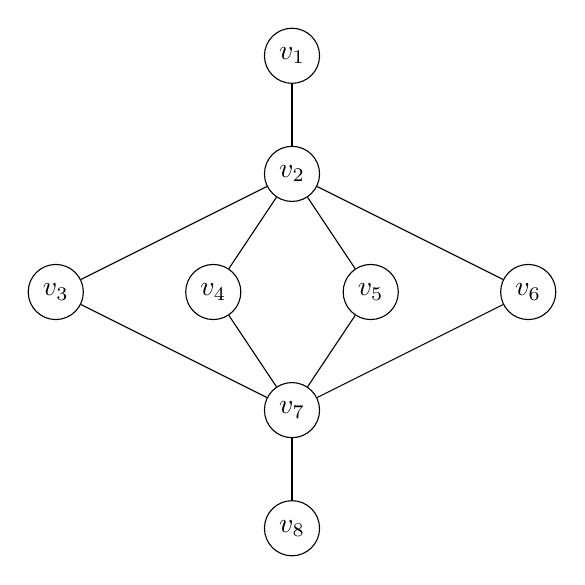
\begin{tikzpicture}[
    % Definimos el estilo de los nodos para no repetir código
    node/.style={circle, draw, minimum size=0.7cm, inner sep=0pt}
  ]

  % 1. Definimos los nodos centrales (v1, v2, v7, v8)
  \node[node] (v1) at (0, 3)  {$v_1$};
  \node[node] (v2) at (0, 1.5) {$v_2$};
  \node[node] (v7) at (0, -1.5) {$v_7$};
  \node[node] (v8) at (0, -3) {$v_8$};

  % 2. Definimos los nodos del medio (v3, v4, v5, v6)
  %Se crean de manera simetrica con el eje y
  \node[node] (v3) at (-3, 0) {$v_3$};
  \node[node] (v4) at (-1, 0) {$v_4$};
  \node[node] (v5) at (1, 0)  {$v_5$};
  \node[node] (v6) at (3, 0)  {$v_6$};

  % 3. Dibujamos las conexiones (Edges)
  \draw (v1) -- (v2);
  \draw (v7) -- (v8);

  % Conexiones desde v2 a los nodos intermedios
  \draw (v2) -- (v3);
  \draw (v2) -- (v4);
  \draw (v2) -- (v5);
  \draw (v2) -- (v6);

  % Conexiones desde v7 a los nodos intermedios
  \draw (v7) -- (v3);
  \draw (v7) -- (v4);
  \draw (v7) -- (v5);
  \draw (v7) -- (v6);

\end{tikzpicture}
En este caso vamos proponer 2 gráficas y el resto son isomorfas de estas.\\
Sean $G_1,G_2 \subseteq G$, Con $G$ siendo la gráfica de arriba.\\
$G_1$: \\
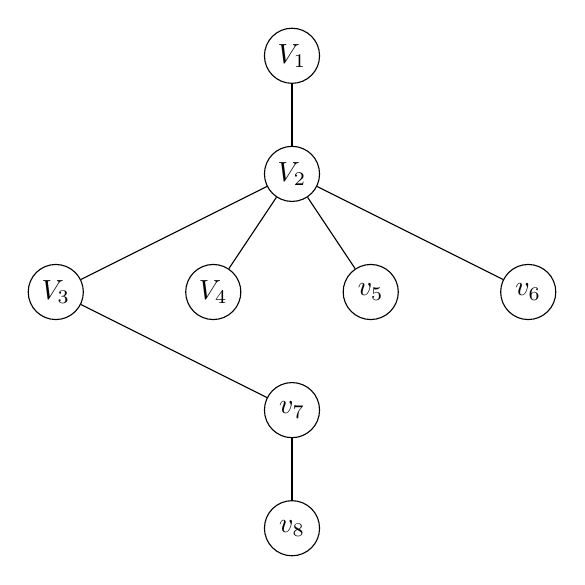
\begin{tikzpicture} %Grafica 1
  [
    % Definimos el estilo de los nodos para no repetir código
    node/.style={circle, draw, minimum size=0.7cm, inner sep=0pt}
  ]
  \node[node] (v1) at (0,3) {$V_1$};
  \node[node] (v2) at (0,1.5) {$V_2$} ;
  \node[node] (v7) at (0, -1.5)  {$v_7$};
  \node[node] (v8) at (0, -3)  {$v_8$};
  \node[node] (v3) at (-3,0) {$V_3$};
  \node[node] (v4) at (-1,0) {$V_4$} ;
  \node[node] (v5) at (1, 0)  {$v_5$};
  \node[node] (v6) at (3, 0)  {$v_6$};
  \draw (v1) -- (v2);
  \draw(v7) -- (v8);
  \draw (v3) -- (v7);
  \draw (v3) -- (v2);
  \draw (v4) -- (v2);
  \draw (v2) -- (v5);
  \draw (v6) -- (v2);
  
\end{tikzpicture}
\newpage $G_2$: \\
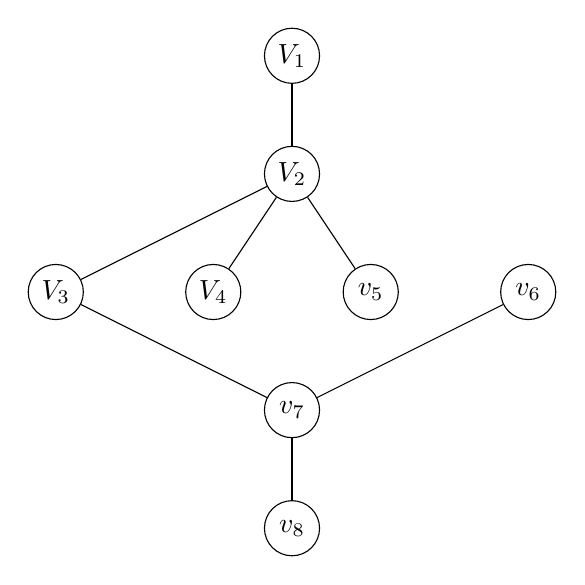
\begin{tikzpicture} %Grafica 1
  [
    % Definimos el estilo de los nodos para no repetir código
    node/.style={circle, draw, minimum size=0.7cm, inner sep=0pt}
  ]
  \node[node] (v1) at (0,3) {$V_1$};
  \node[node] (v2) at (0,1.5) {$V_2$} ;
  \node[node] (v7) at (0, -1.5)  {$v_7$};
  \node[node] (v8) at (0, -3)  {$v_8$};
  \node[node] (v3) at (-3,0) {$V_3$};
  \node[node] (v4) at (-1,0) {$V_4$} ;
  \node[node] (v5) at (1, 0)  {$v_5$};
  \node[node] (v6) at (3, 0)  {$v_6$};
  \draw (v1) -- (v2);
  \draw(v7) -- (v8);
  \draw (v3) -- (v7);
  \draw (v3) -- (v2);
  \draw (v4) -- (v2);
  \draw (v2) -- (v5);
  \draw (v6) -- (v7);
  
\end{tikzpicture}
\\ En este caso con $G_1$ y $G_2$ basta para formar a las demás subgráficas debido a que son isomorfas de estos dos.
Dado que $v_1$ solo puede estar conectado a $v_2$ y $v_8$ solo puede estar conectado a $v_7$, esas aristas estaran en todo arbol generador. \\
En el caso de las demás aristas, al ser simetricas sus conexiones, entonces cualquier combinación se puede hacer con ellas de manera similar,
y aun mantendrían su forma de árbol generador.
\end{justify}

\end{document} %Fin del documento
